\section{Run Kallisto on a single
sample}\label{run-kallisto-on-a-single-sample}

expVIP can run \lstinline!Kallisto! and load the \lstinline!tpm! and
\lstinline!counts! to the database. The only requirement is to run
\lstinline!kallisto index! on the transcriptome reference.

\subsection{Graphical interface}\label{graphical-interface}

\begin{enumerate}
\def\labelenumi{\arabic{enumi}.}
\itemsep1pt\parskip0pt\parsep0pt
\item
  Double click on \lstinline!run_kallisto.sh!
  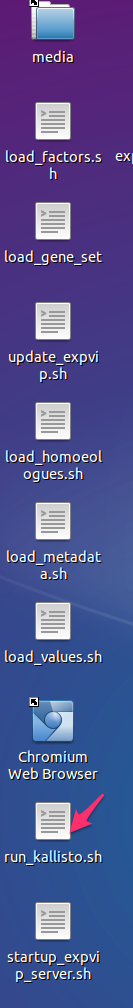
\includegraphics{images/RunKallisto01.png}
\item
  Click on \lstinline!Execute on terminal!
  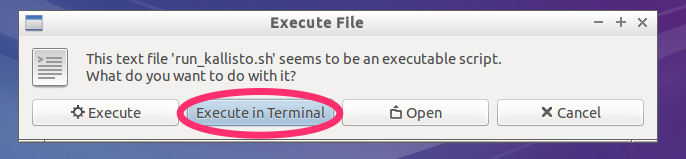
\includegraphics{images/RunKallisto02.png}
\item
  Give a name to the set of mappings to be grouped. All mappings done
  with the same reference and preference should have the same name.
  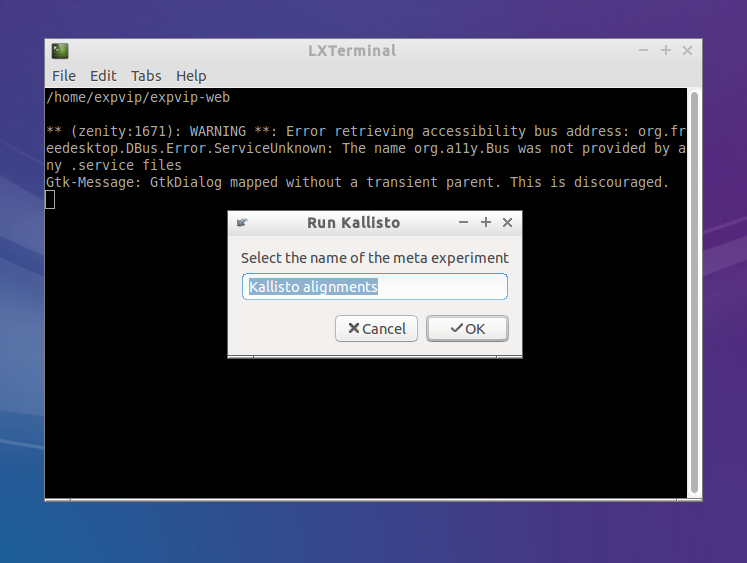
\includegraphics{images/RunKallisto03.png}
\item
  Get the name of the reference. This name must be the same used when
  loading the \href{LoadingMetadata}{metadata}
  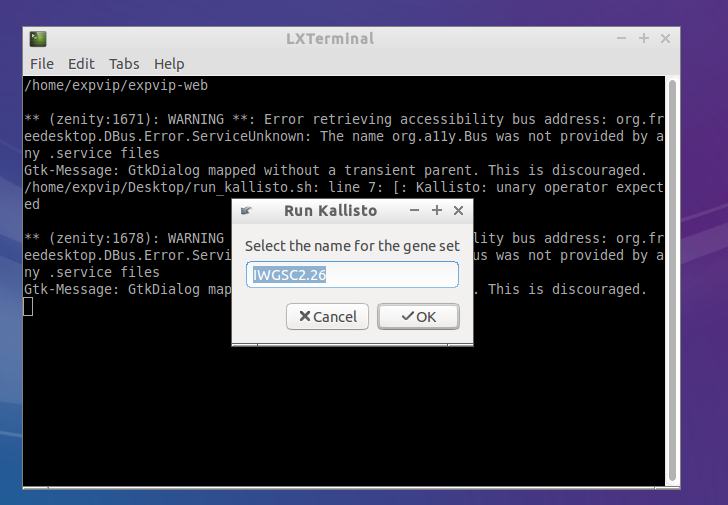
\includegraphics{images/RunKallisto04.png}
\item
  Select a folder with the reads. The reads must be paired reads. The
  folder name must be the same as the \lstinline!accession! used on the
  metadata. 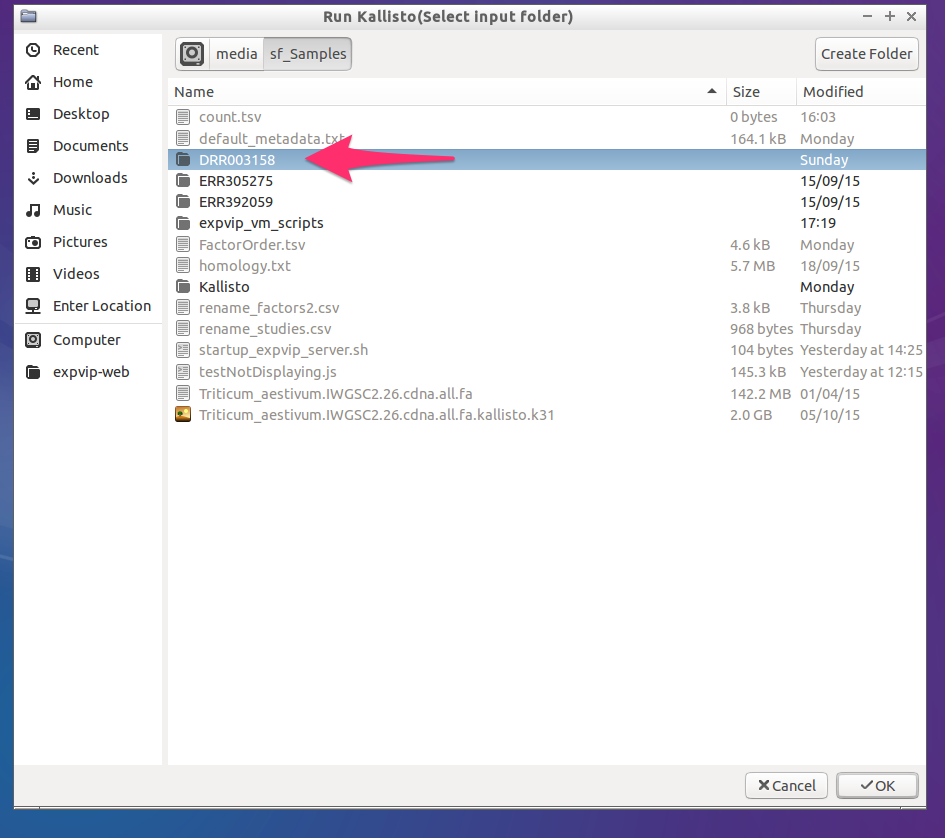
\includegraphics{images/RunKallisto05.png}
\item
  Select the kallisto index 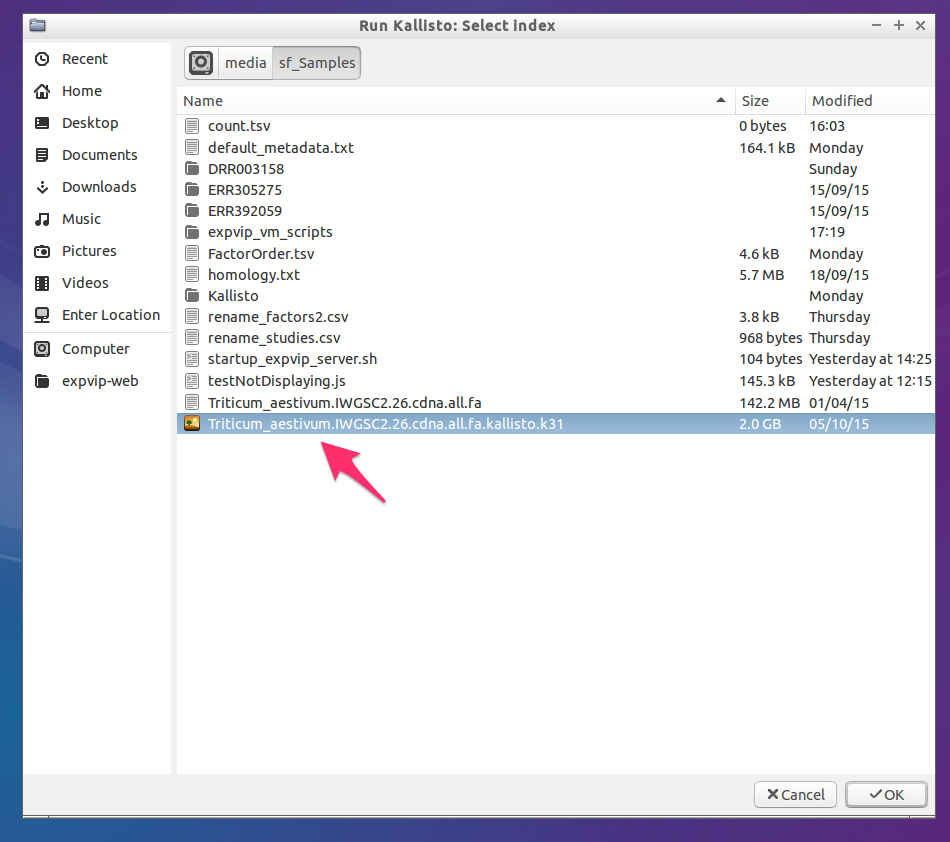
\includegraphics{images/RunKallisto07.png}
\item
  Wait for Kallisto to run and load the data
  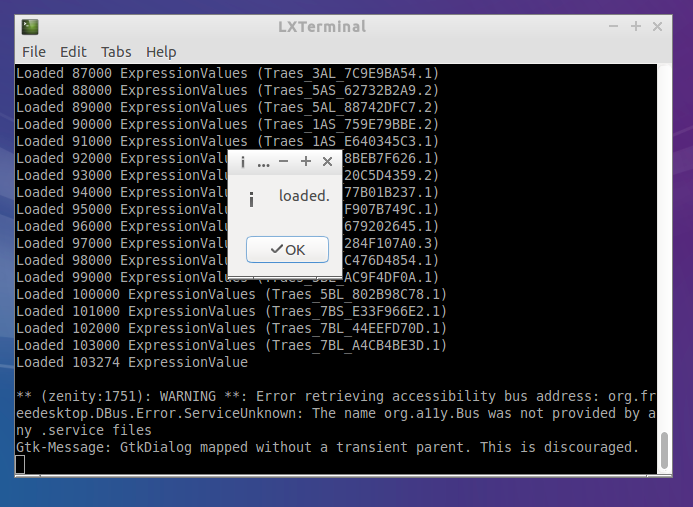
\includegraphics{images/RunKallisto08.png}
\end{enumerate}

You can repeat this with all the samples or you can use the
\href{RunKallistoBatch}{batch load}.

\subsection{Rake task}\label{rake-task}

\begin{lstlisting}[language=sh]
kallisto:runAndStorePaired[kallistoIndex,input_folder,metaExperimentName,geneSetName]
\end{lstlisting}

Where \lstinline!metaExperimentName! is the name of the group of
alignments under the same conditions and `\lstinline!geneSetName! is the
name of the reference.
